\documentclass{article}

\usepackage[paper=letterpaper,margin=2.5cm]{geometry} % Set Margins

%% Math and math fonts
\usepackage{amsmath, amsthm, amssymb, amsfonts}
\usepackage{bbm} % for \mathbbm{1}

% date
\usepackage[nodayofweek]{datetime}

% Color
\usepackage{color, xcolor}

% Misc
\usepackage{environ}  % \collect@body in asmmath
\usepackage{graphicx} % \includegraphics options
\usepackage{mdframed} % text boxes
\usepackage{indentfirst} % Indent first paragraph after section header
\usepackage[shortlabels]{enumitem} % Control enumerate items with [(a)]
\usepackage{comment} % Comments
\usepackage{fancyhdr} % Headers and footers

% Tables
\usepackage{array}

% Sub-figures and figure placement
\usepackage{caption}
\usepackage{subcaption}
\usepackage{float} 

% Graphing
\usepackage{pgfplots}
\pgfplotsset{compat=1.17}
\usepackage{tikz}

% Title Placement
\usepackage{titling}
\setlength{\droptitle}{-6em}

%set indent to 
\setlength{\parindent}{0pt}

% Hyper refs
\usepackage{hyperref}
\hypersetup{
    colorlinks=true,
    linkcolor=blue,
    urlcolor  = blue,
    filecolor=magenta,      
    urlcolor=blue,
    citecolor = blue,
    anchorcolor = blue
}

% % Citation management
\usepackage{natbib}
\bibliographystyle{abbrvnat}
\setcitestyle{authordate,open={(},close={)}}

\pagestyle{fancy}

\usepackage[paper=letterpaper,margin=2.5cm]{geometry} % Set Margins

%% Math and math fonts
\usepackage{amsmath, amsthm, amssymb, amsfonts}
\usepackage{bbm} % for \mathbbm{1}

% date
\usepackage[nodayofweek]{datetime}

% Color
\usepackage{color, xcolor}

% Misc
\usepackage{environ}  % \collect@body in asmmath
\usepackage{graphicx} % \includegraphics options
\usepackage{mdframed} % text boxes
\usepackage{indentfirst} % Indent first paragraph after section header
\usepackage[shortlabels]{enumitem} % Control enumerate items with [(a)]
\usepackage{comment} % Comments
\usepackage{fancyhdr} % Headers and footers

% Tables
\usepackage{array}

% Sub-figures and figure placement
\usepackage{caption}
\usepackage{subcaption}
\usepackage{float} 

% Graphing
\usepackage{pgfplots}
\pgfplotsset{compat=1.17}
\usepackage{tikz}

% Title Placement
\usepackage{titling}
\setlength{\droptitle}{-6em}

%set indent to 
\setlength{\parindent}{0pt}

% Hyper refs
\usepackage{hyperref}
\hypersetup{
    colorlinks=true,
    linkcolor=blue,
    urlcolor  = blue,
    filecolor=magenta,      
    urlcolor=blue,
    citecolor = blue,
    anchorcolor = blue
}

% % Citation management
\usepackage{natbib}
\bibliographystyle{abbrvnat}
\setcitestyle{authordate,open={(},close={)}}

% ----------------------------------------
% TITLE
% ----------------------------------------

\pagestyle{fancy}

\lhead{Creel}
\chead{Week Two}
\rhead{AMES}

\title{AMES Class Notes}
\author{Andie Creel}

\begin{document}
\maketitle



\section{Level Sets}
You can think of level sets as a contour map of a mountain. It's a flat map, but the circles around the peak denote the elevation. This is a hiking example, but you could think about maximizing utility. Each level set would be a utility level. If you're trying to maximize utility, you'd want to be on the level set associated with the highest level of utility. 

\begin{figure}[htp]
    \centering
        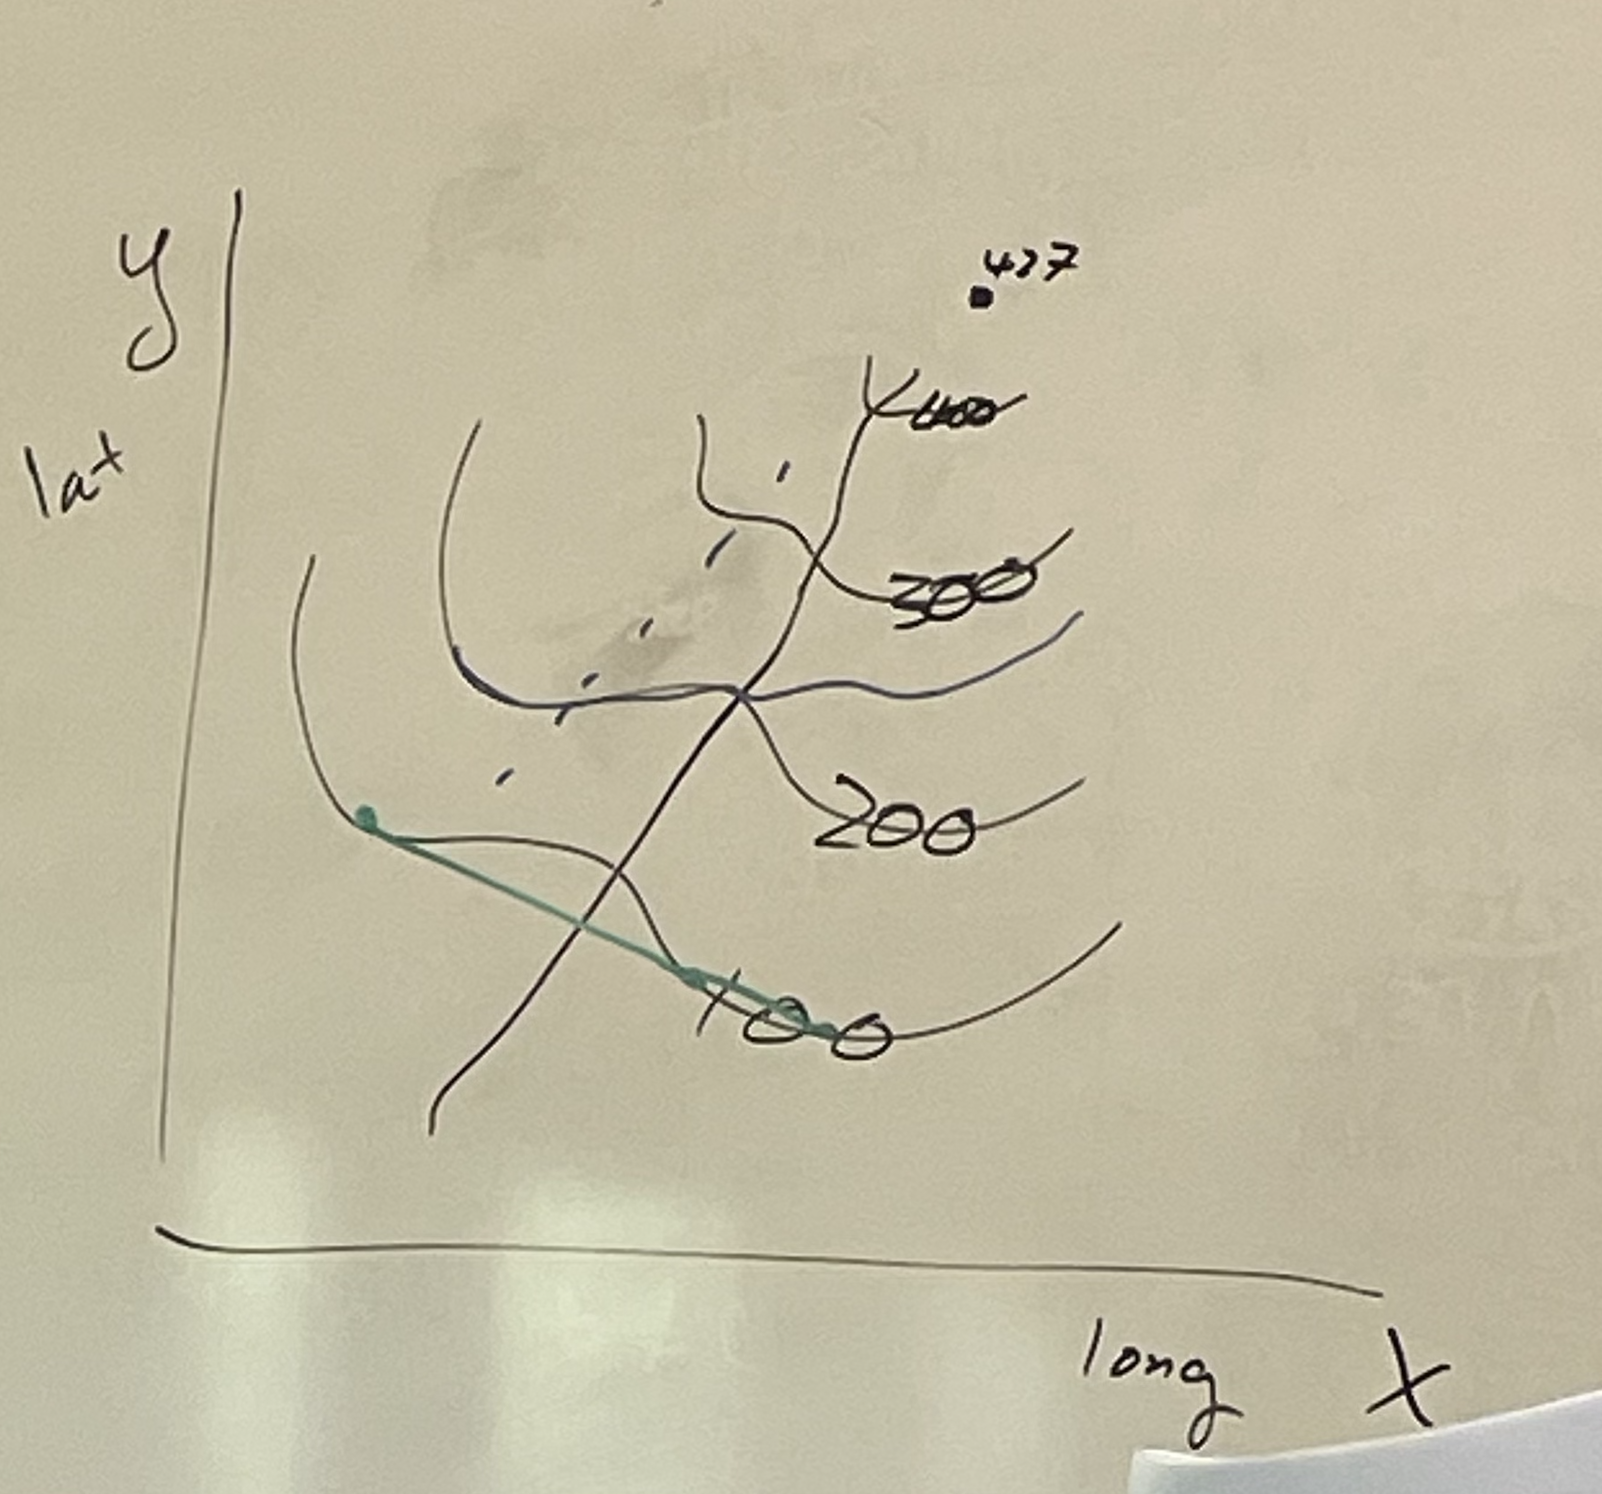
\includegraphics[width=0.5\textwidth]{Screen Shot 2023-09-06 at 10.57.01 AM.png}
    \caption{Level sets}
    \label{fig:sample}
\end{figure}

\section{Solving a system of equations}

Solution to many problems is to find where two lines meet. 

\begin{align}
    P = a-bQ \\
    P = w +yQ\\
    S = D = Q
\end{align}

set two equations equal to one another because $P = P$ and solve for Q
\begin{align}
    a - bQ = w + yQ \\
    a - w = yQ + bQ \\
    a - w = (y+b) Q\\
    Q = \frac{a - w}{y + b}
\end{align}

\subsection{Problem set example}

In the problem set, you'll see:

\begin{align}
    \frac{\partial a}{\partial t} = ar_a (1 - \frac{a + \alpha b}{K_a}) = 0\\
    \frac{\partial b}{\partial t} = br_b (1 - \frac{\beta a + b }{K_b}) = 0
\end{align}

We know that we're looking for an \textbf{equilibrium} (\textit{i.e., } where the system isn't changing) and so the \textit{derivatives  equal to zero}. \\

In the above example, what are we solving for? The values of $a$ and $b$ (those are what change through time $t$, they are our variables). \\

How many solutions do we expect to have for $a$ and $b$? 2 for each, because equation 8 and equation 9 are both quadratic equations with respect to $a$ and $b$, respectively. Therefore, we would expect to have two "roots" for each. Recall that a root is the value of your variable that would cause your equation to evaluate to zero. \\

Because there is two solutions for $a$ where eqn 8 = 0, and two solutions for $b$ where eqn 9 = 0 then there are four potential solutions as sets of $(a,b)$. Immediately we can tell that $a= 0$ and $b = 0$ will be a solution to eqn 8 and 9, because of the zero multiplicative rule and a and b being in the first multiplicative term. \\

Own solutions are going to take the form of $(a, b)$. 
\begin{align}
    (0, 0) \\
    (?, 0) \\
    (0, ?) \\
    (?, ?)
\end{align}

If we want to fill in the question mark of 11, we can take eqn 8 
\begin{align*}
    \frac{\partial a}{\partial t} = ar_a (1 - \frac{a + \alpha b}{K_a}) = 0 \\
    1 - \frac{a + \alpha b}{K_a} = 0 \\ 
    1 - \frac{a}{K_\alpha} = 0\\
    a = K_a
\end{align*}
Because of the zero multiplicative rule, then that we know b = 0,  then some simple algebra. 


We can do the exact same thing for eqn 12 and get the following solutions: 
\begin{align}
    (0, 0) \\
    (K_a, 0) \\
    (0, K_b) \\
    (?, ?)
\end{align}

For the final solution we have two equations and two unknowns (these come from our original eqns 8 and 9 after using the 0 multiplicative rule and then moving the 1 to the other side): 

\begin{align}
    1 = \frac{a + \alpha b}{K_a} \\
    1 = \frac{\beta a + b }{K_b}
\end{align}

We can now solve for a in eqn 18, plug that solution into 19 and solve for b. We can the solution for b into 18 to get our solution for a. This will give us our final solution.  \\

\textit{An algebra tip:} We are solving for $a$ and $b$. If we find messy terms that \textbf{don't} have an $a$ or $b$, we can relabel those terms because those terms are just a constant that we can name. This really helps simplify the algebra. 

\section{Quadratic Formula and relabeling}

Let's say you have a quadratic equation 
\begin{align}
    y = a x^2 + bx + d
\end{align}

Recall, you can only use the quadratic formula if the equation is equal to zero!! 

\begin{align}
    0 = = a x^2 + bx + d - y
\end{align}

But now this is not in the familiar form we know for the quadratic formula. Let $c = d-y$. \textit{This means that we're holding $y$ fixed. We chose to do this as the modeler. We have chosen to hold $y$ constant, implicitly.} \\

We can rewrite our equation: 
\begin{align}
    0 = a x^2 + bx + c
\end{align}

and so we can now solve for the roots of $x$ using the quadratic formal  
\[x = \frac{-b \pm \sqrt{b^2 - 4ac}}{2a}\]


\section{Trig Functions}

Trig functions don't work in an $(x,y)$ space. They work in a \textit{polar} space $(r, \theta)$, where $r$ is a radial distance for the origin and $\theta$ is the angle for the x axis.  They do get used a lot in applied settings, but don't let them scare you. \\

\textbf{Key point:} If you see these, you should think about circles. 

\begin{figure}[htp]
    \centering
        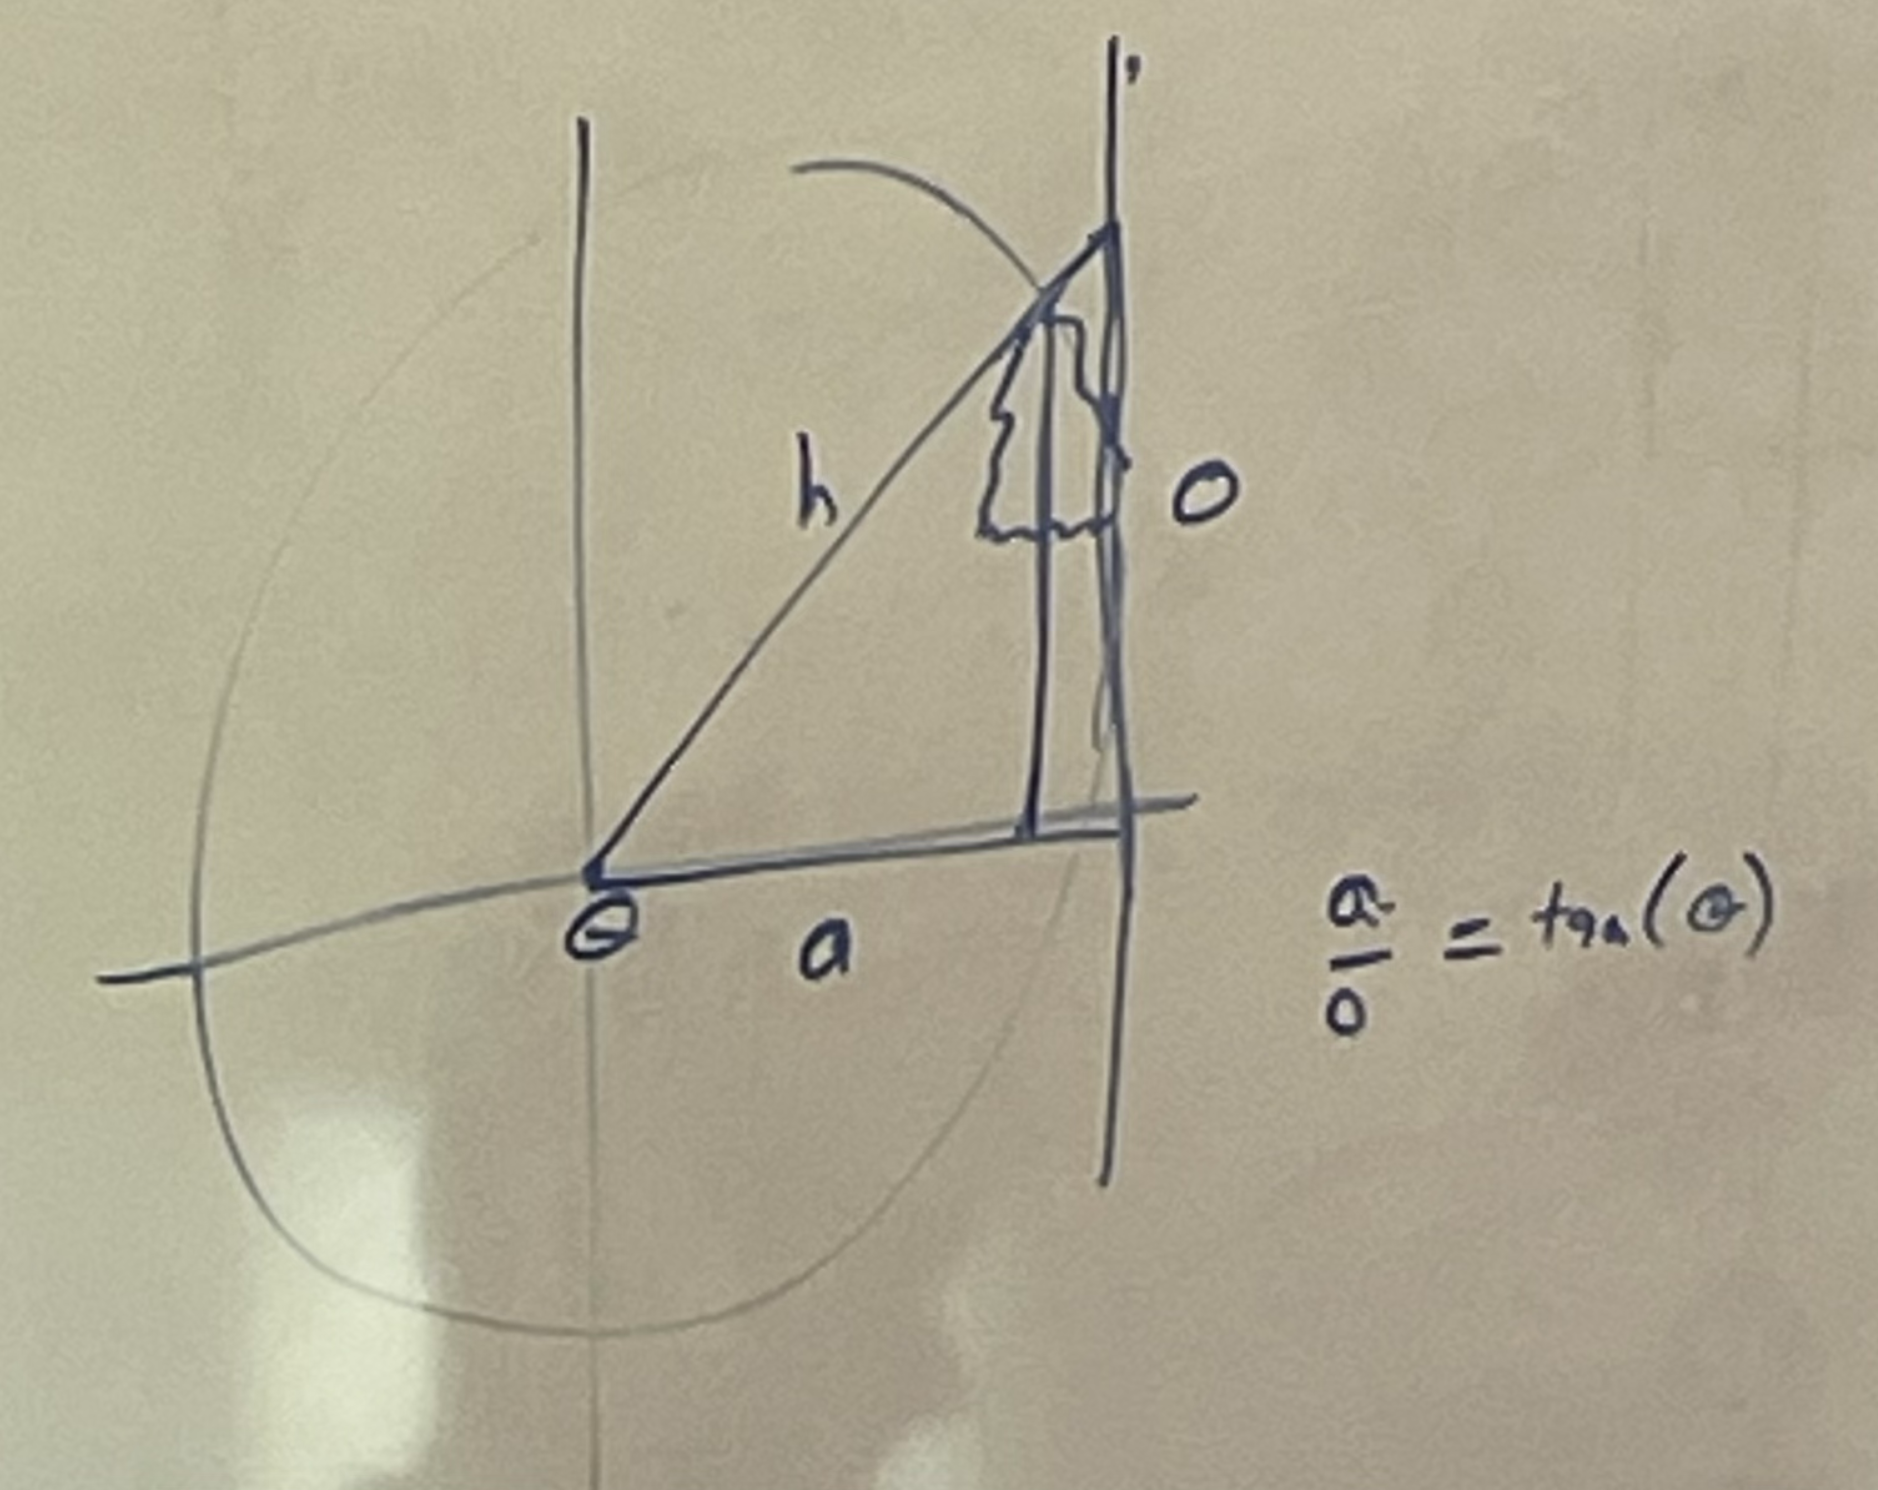
\includegraphics[width=0.5\textwidth]{Screen Shot 2023-09-06 at 11.29.46 AM.png}
    \caption{Trig}
\end{figure}

\begin{align}
    \sin(\theta) = \frac{o}{h}\\
    \cos(\theta) = \frac{a}{h} \\
    \tan(\theta) = \frac{o}{a}
\end{align}

A rhyme to remember this: Soh Cah Toa. 

\section{Expectation function}
The expectation function is the average
\begin{align}
    E(x_n) = \frac{1}{N} \sum_n x_n
\end{align}


\section{Jensen's Inequality}

Let $F(x)$ and $G(x)$ both be \textbf{non-linear} equations. Most environmental models involve \textit{lots} of non-linear equations. Then Jensen's inequality tells us that 
\begin{align}
    F(G(X)) \neq G(F(X)).
\end{align}

The Jensen's inequality applies to the expectation operator 
\begin{align}
    E(F(X)) \neq F(E(X))
\end{align}

\subsection{showing this is true}

Let our set of $X$ be:
\begin{align}
    X = \{1, 2, 3, 4, 5\}
\end{align}

And 
\begin{align}
    F(x) = x^2
\end{align}

The right hand side of this special case of Jensen inequality:
\begin{align}
    F(E(X)) = F(E(\{1, 2, 3, 4, 5\}))\\
    = F(3) \\
    = 3^2 \\
    = 9
\end{align}

The left hand side of this special case of Jensen is 
\begin{align}
    E(F(X)) = E(X^2) \\
    = E(\{1, 4, 9, 16, 25\}) \\
    = 11
\end{align}

and so 
\begin{align}
    E(F(X)) \neq F(E(X))\\
    11 \neq 9
\end{align}

\section{Units}

PAY ATTENTION TO UNITS! You will be working with many people in many spaces. Make sure you're all working with the same units. The reason you may be taking past one another may be as simple as you and the other person are using different units and you don't even know that yet. 

If you have the equation: 
\begin{align}
    y = a + bx
\end{align}

then $y$, $a$ and $bx$ need to all be in the same unit. $b$ is in the unit of $\frac{a}{x}$.\\

In the climate conversation we know our units (tons of green house gas equivalent emissions). However, in biodiversity we don't know the units yet. In environmental justice conversations, we don't always know the unit. And so when we're trying to maximize benefit or minimize harm, we don't totally know how if we don't know the unit. \\

If you only get one thing out of this class, \textbf{pay attention to units}. 

\section{Concave and Convex \textit{Functions}}
Last week we talked about concave and convex set, and why they are important for tipping points.\\

Concavity and convexity mean something different for \textit{functions} than it does for \textit{sets.}

\begin{figure}[htp]
    \centering
        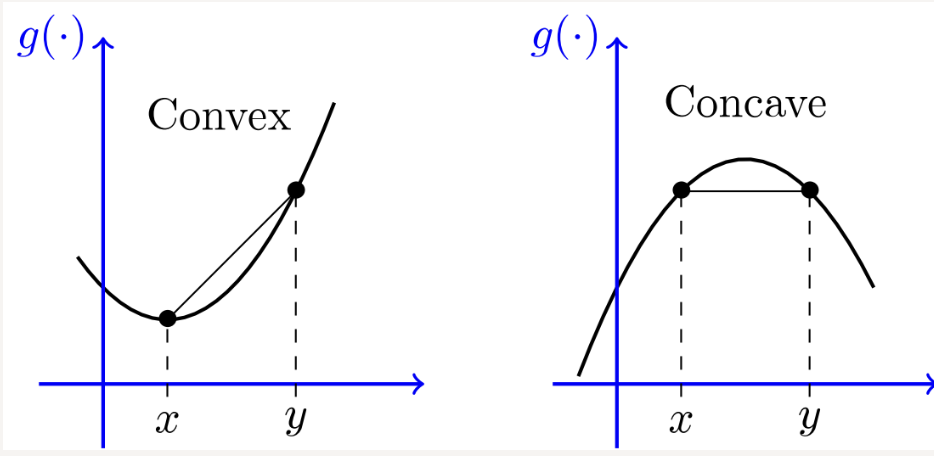
\includegraphics[width=0.5\textwidth]{Screen Shot 2024-09-09 at 10.45.31 AM.png}
    \caption{Convex and concave functions}
    \label{fig:sample}
\end{figure}

\textbf{Quasi-concave:} Describes a 3+ dimensional function where the level sets (what the function looks like in 2 dimension) is convex. This is important in welfare economics and utility maximization problems. If a function is quasi-concave, it has useful properties for utility maximization. 



\end{document}